% RMS Gantt chart — tau1(C=1,T=4) tau2(C=2,T=8) tau3(C=3,T=16) over [0,16]
% RMS priority order: tau1 > tau2 > tau3 (shorter period = higher priority)
% tau3 is preempted at t=4 by tau1; resumes at t=5.
\documentclass[border=5pt]{standalone}
\usepackage{lmodern}
\usepackage{tikz}
\usetikzlibrary{arrows.meta,patterns}

\definecolor{kmblue}{HTML}{003874}
\definecolor{kmgold}{HTML}{BA9224}
\definecolor{rtgreen}{HTML}{1F9D55}
\definecolor{rtred}{HTML}{E3342F}
\definecolor{axgray}{HTML}{888888}
\definecolor{dkgray}{HTML}{555555}

\begin{document}
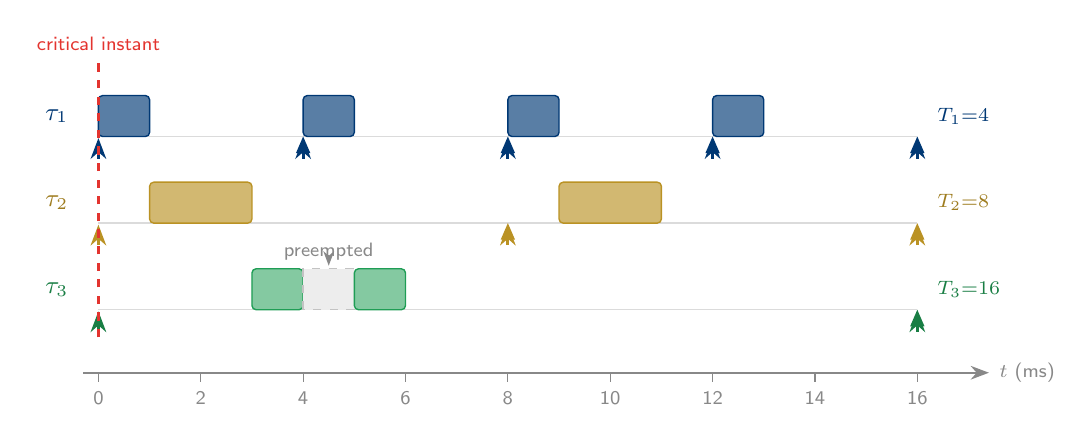
\begin{tikzpicture}[>=Stealth,font=\sffamily,x=0.65cm,y=1cm]

  \def\h{0.52}   % block height
  \def\ra{3.0}   % tau1 row y-base
  \def\rb{1.9}   % tau2 row y-base
  \def\rc{0.8}   % tau3 row y-base

  % ---- time axis ----
  \draw[axgray,line width=0.8pt,->] (-0.3,0) -- (17.4,0)
        node[right,font=\sffamily\scriptsize] {$t$ (ms)};
  \foreach \t in {0,2,4,6,8,10,12,14,16} {
    \draw[axgray] (\t,0) -- (\t,-0.12)
          node[below,font=\sffamily\scriptsize,axgray] {\t};
  }

  % ---- row baseline guides ----
  \foreach \y in {\ra,\rb,\rc}
    \draw[axgray!30,line width=0.5pt] (0,\y) -- (16,\y);

  % ---- task labels ----
  \node[anchor=east,kmblue,font=\sffamily\small\bfseries]
        at (-0.4,\ra+0.5*\h) {$\tau_1$};
  \node[anchor=east,kmgold!85!black,font=\sffamily\small\bfseries]
        at (-0.4,\rb+0.5*\h) {$\tau_2$};
  \node[anchor=east,rtgreen!80!black,font=\sffamily\small\bfseries]
        at (-0.4,\rc+0.5*\h) {$\tau_3$};

  % ---- tau1 blocks [0,1] [4,5] [8,9] [12,13] ----
  \foreach \s/\e in {0/1, 4/5, 8/9, 12/13} {
    \fill[kmblue!65,rounded corners=1.5pt]
          (\s,\ra) rectangle (\e,\ra+\h);
    \draw[kmblue,line width=0.5pt,rounded corners=1.5pt]
          (\s,\ra) rectangle (\e,\ra+\h);
  }

  % ---- tau2 blocks [1,3] [9,11] ----
  \foreach \s/\e in {1/3, 9/11} {
    \fill[kmgold!65,rounded corners=1.5pt]
          (\s,\rb) rectangle (\e,\rb+\h);
    \draw[kmgold,line width=0.5pt,rounded corners=1.5pt]
          (\s,\rb) rectangle (\e,\rb+\h);
  }

  % ---- tau3 blocks: [3,4] then preempted gap [4,5] then [5,6] ----
  \fill[rtgreen!55,rounded corners=1.5pt]
        (3,\rc) rectangle (4,\rc+\h);
  \draw[rtgreen,line width=0.5pt,rounded corners=1.5pt]
        (3,\rc) rectangle (4,\rc+\h);
  % preemption gap [4,5] — hatched grey
  \fill[axgray!15] (4,\rc) rectangle (5,\rc+\h);
  \draw[axgray!50,line width=0.5pt,dashed] (4,\rc) rectangle (5,\rc+\h);
  \fill[rtgreen!55,rounded corners=1.5pt]
        (5,\rc) rectangle (6,\rc+\h);
  \draw[rtgreen,line width=0.5pt,rounded corners=1.5pt]
        (5,\rc) rectangle (6,\rc+\h);

  % ---- release arrows (upward from row base) ----
  \foreach \t in {0,4,8,12,16}
    \draw[kmblue,line width=1.0pt,->]
          (\t,\ra-0.28) -- (\t,\ra-0.02);
  \foreach \t in {0,8,16}
    \draw[kmgold,line width=1.0pt,->]
          (\t,\rb-0.28) -- (\t,\rb-0.02);
  \foreach \t in {0,16}
    \draw[rtgreen!80!black,line width=1.0pt,->]
          (\t,\rc-0.28) -- (\t,\rc-0.02);

  % ---- deadline marks (inverted triangle at row base) ----
  \foreach \t in {4,8,12,16}
    \fill[kmblue] (\t,\ra) -- (\t-0.14,\ra-0.21) -- (\t+0.14,\ra-0.21) -- cycle;
  \foreach \t in {8,16}
    \fill[kmgold] (\t,\rb) -- (\t-0.14,\rb-0.21) -- (\t+0.14,\rb-0.21) -- cycle;
  \fill[rtgreen!80!black]
        (16,\rc) -- (15.86,\rc-0.21) -- (16.14,\rc-0.21) -- cycle;

  % ---- critical instant annotation ----
  \draw[rtred,dashed,line width=0.9pt]
        (0,\rc-0.35) -- (0,\ra+\h+0.45);
  \node[rtred,font=\sffamily\scriptsize,above] at (0,\ra+\h+0.45)
        {critical instant};

  % ---- preemption annotation ----
  \node[axgray,font=\sffamily\scriptsize] at (4.5,\rc+\h+0.22)
        {preempted};
  \draw[axgray,line width=0.5pt,->]
        (4.5,\rc+\h+0.18) -- (4.5,\rc+\h+0.04);

  % ---- period labels on right ----
  \node[kmblue,font=\sffamily\scriptsize,anchor=west]
        at (16.2,\ra+0.5*\h) {$T_1{=}4$};
  \node[kmgold!85!black,font=\sffamily\scriptsize,anchor=west]
        at (16.2,\rb+0.5*\h) {$T_2{=}8$};
  \node[rtgreen!80!black,font=\sffamily\scriptsize,anchor=west]
        at (16.2,\rc+0.5*\h) {$T_3{=}16$};


\end{tikzpicture}
\end{document}
